\documentclass{beamer}
% Prévoir à peu près un transparent par minute d'exposé.
% Deux ou trois sections semble être une bonne chose.
\mode<presentation>
{
	\usetheme{Warsaw}
	\setbeamercovered{highly dynamic}
	\setbeamercovered{invisible}
}

\usepackage[english]{babel}
\usepackage[utf8]{inputenc}
%\usepackage{hyperref}

\setbeamersize{text margin left=20pt}
\setbeamersize{text margin right=20pt}

\defbeamertemplate*{footline}{infolines theme}
{
	\leavevmode%
	\hbox{%
		\begin{beamercolorbox}[wd=.5\paperwidth,ht=2.25ex,dp=1ex,center]{author in head/foot}%
			\usebeamerfont{author in head/foot}G. Lesauvage
		\end{beamercolorbox}%
		\begin{beamercolorbox}[wd=.25\paperwidth,ht=2.25ex,dp=1ex,center]{title in head/foot}%
			\usebeamerfont{title in head/foot}\insertshorttitle
		\end{beamercolorbox}%
		\begin{beamercolorbox}[wd=.25\paperwidth,ht=2.25ex,dp=1ex,right]{date in head/foot}%
			\usebeamerfont{date in head/foot}june 29th, 2009\hspace*{2em}
			\insertframenumber{}/\inserttotalframenumber\hspace*{2ex}
		\end{beamercolorbox}
	}%
	\vskip0pt%
}

\date{june 29th, 2009}
\title[ICCSA 2009]
{
	Dynamical Handling of Straddle Carriers Activities on a Container Terminal in an Uncertain Environment\\
	- Swarm Intelligence Approach -
}

\author
{
	S. Balev \and F. Guinand \and \textbf{G. Lesauvage} \and D. Olivier
}

\institute[UFR ST Le Havre]
{
	\begin{columns}
		\begin{column}[l]{6cm}
			\begin{center}
			
\includegraphics[height=.1\textheight]{../Articles/Figures/logouniversiteduhavre.png} \\
			\textit{Unité de Formation et de Recherche des Sciences et Techniques}
			\end{center}
		\end{column}
		\begin{column}[r]{6cm}
			\begin{center}
			
\includegraphics[height=.1\textheight]{../Articles/Figures/logolitis.png} \\
			\textit{Laboratoire d'Informatique et du Traitement de l'Information et des Systèmes}
			\end{center}
		\end{column}
	\end{columns}

 	
}



 \AtBeginSection[Plan]
 {
 \begin{frame}<beamer>
 
 \frametitle{Outline}
 \tableofcontents[currentsection]
 \end{frame}
 }
\setbeamertemplate{blocks}[rounded][shadow=true]
\subject{ICCSA 2009}
\begin{document}

\begin{frame}
\titlepage
\end{frame}

\begin{frame}
\frametitle{Outline}
\tableofcontents
\end{frame}


\section{System description}
\subsection*{CALAS}
\begin{frame}
\frametitle{The CALAS project}
	\begin{itemize}
 		\item CALAS project : localizing precisely handling trucks on a container terminal
		\item Laser measure system and software
		\item 2 companies : 
			\begin{itemize}
			 \item Laser Data Technology Terminal 
	 		 \item \textit{Terminaux de Normandie}
			\end{itemize}
			
	\end{itemize}
	\begin{block}{Objective of the CALAS project : }
		\begin{minipage}[]{\columnwidth}
			To know the state of the terminal, in real time, for both containers and trucks location.
		\end{minipage}
	\end{block}


\end{frame}
\subsection*{Container Terminal}
\begin{frame}
\frametitle{Terminal description}

 	\begin{columns}
 	 	\begin{column}[l]{6cm}
			\begin{itemize}
				\item Container terminal
				\item 3 main areas : 
				\begin{itemize}
 					\item Ship handling
					\item Stock area
					\item Truck/Train handling
				\end{itemize}
			\end{itemize}
		\end{column}
 	 	\begin{column}[r]{4.7cm}
			\begin{flushright}
				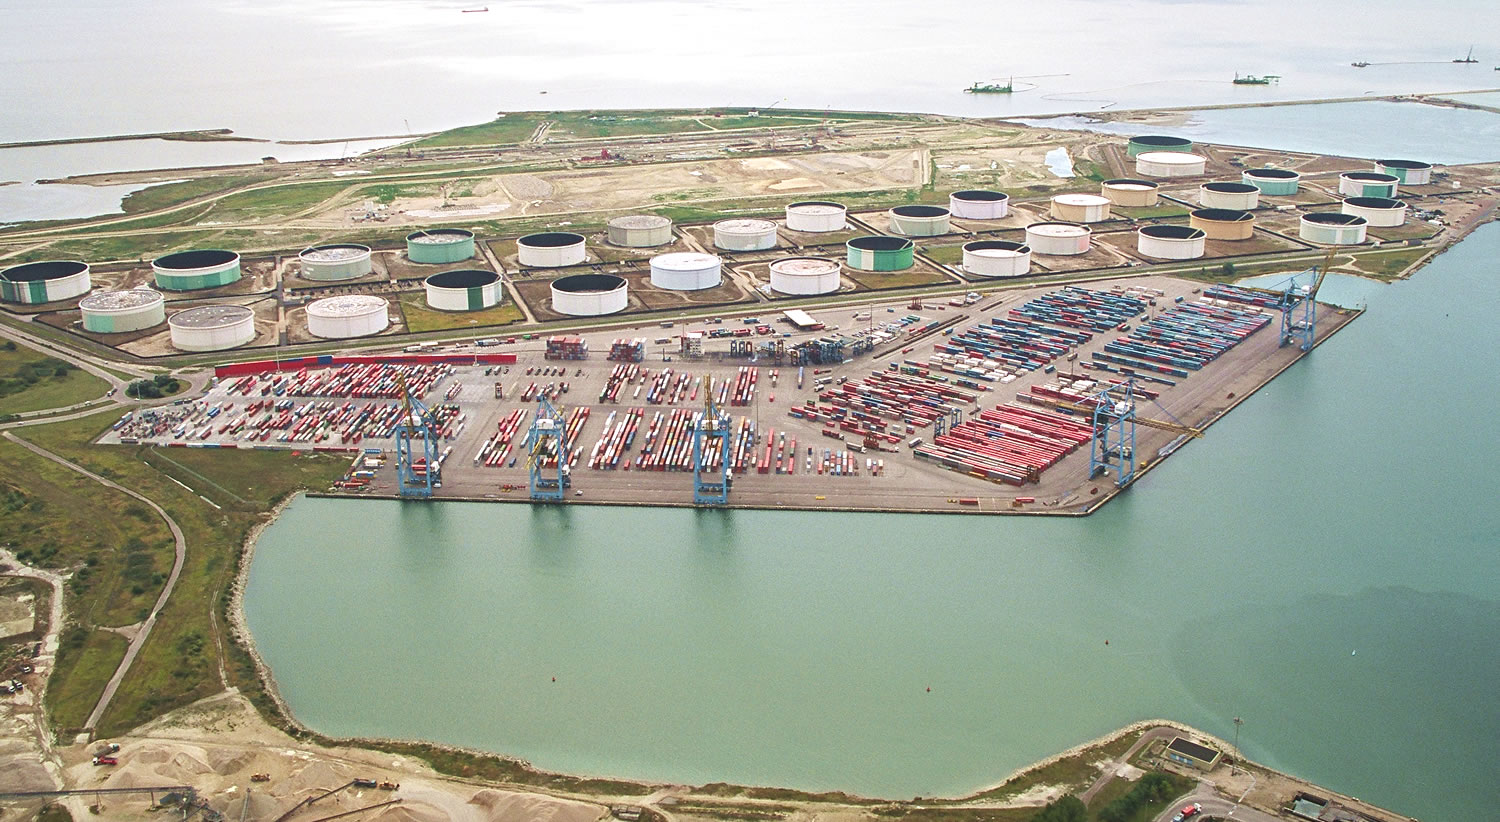
\includegraphics[height=.30\textheight]{../Articles/Figures/terminalDeNormandie.jpg}
			\end{flushright}
		\end{column}
 	\end{columns}

	\begin{columns}
 	 	\begin{column}[l]{8,5cm}
 		\begin{itemize} 
\item Stock area contains many long rows of stacked containers		
\item Straddle carriers have to move containers from a place inside the terminal to another one
		\item 3 kinds of missions : 
			\begin{itemize}
				\item Preparing a ship (un)loading
				\item Preparing a truck (un)loading
				\item Optimizing stock area
			\end{itemize}
	\end{itemize}
	\end{column}
 	 	\begin{column}[r]{2,2cm}
			\begin{flushright}
			    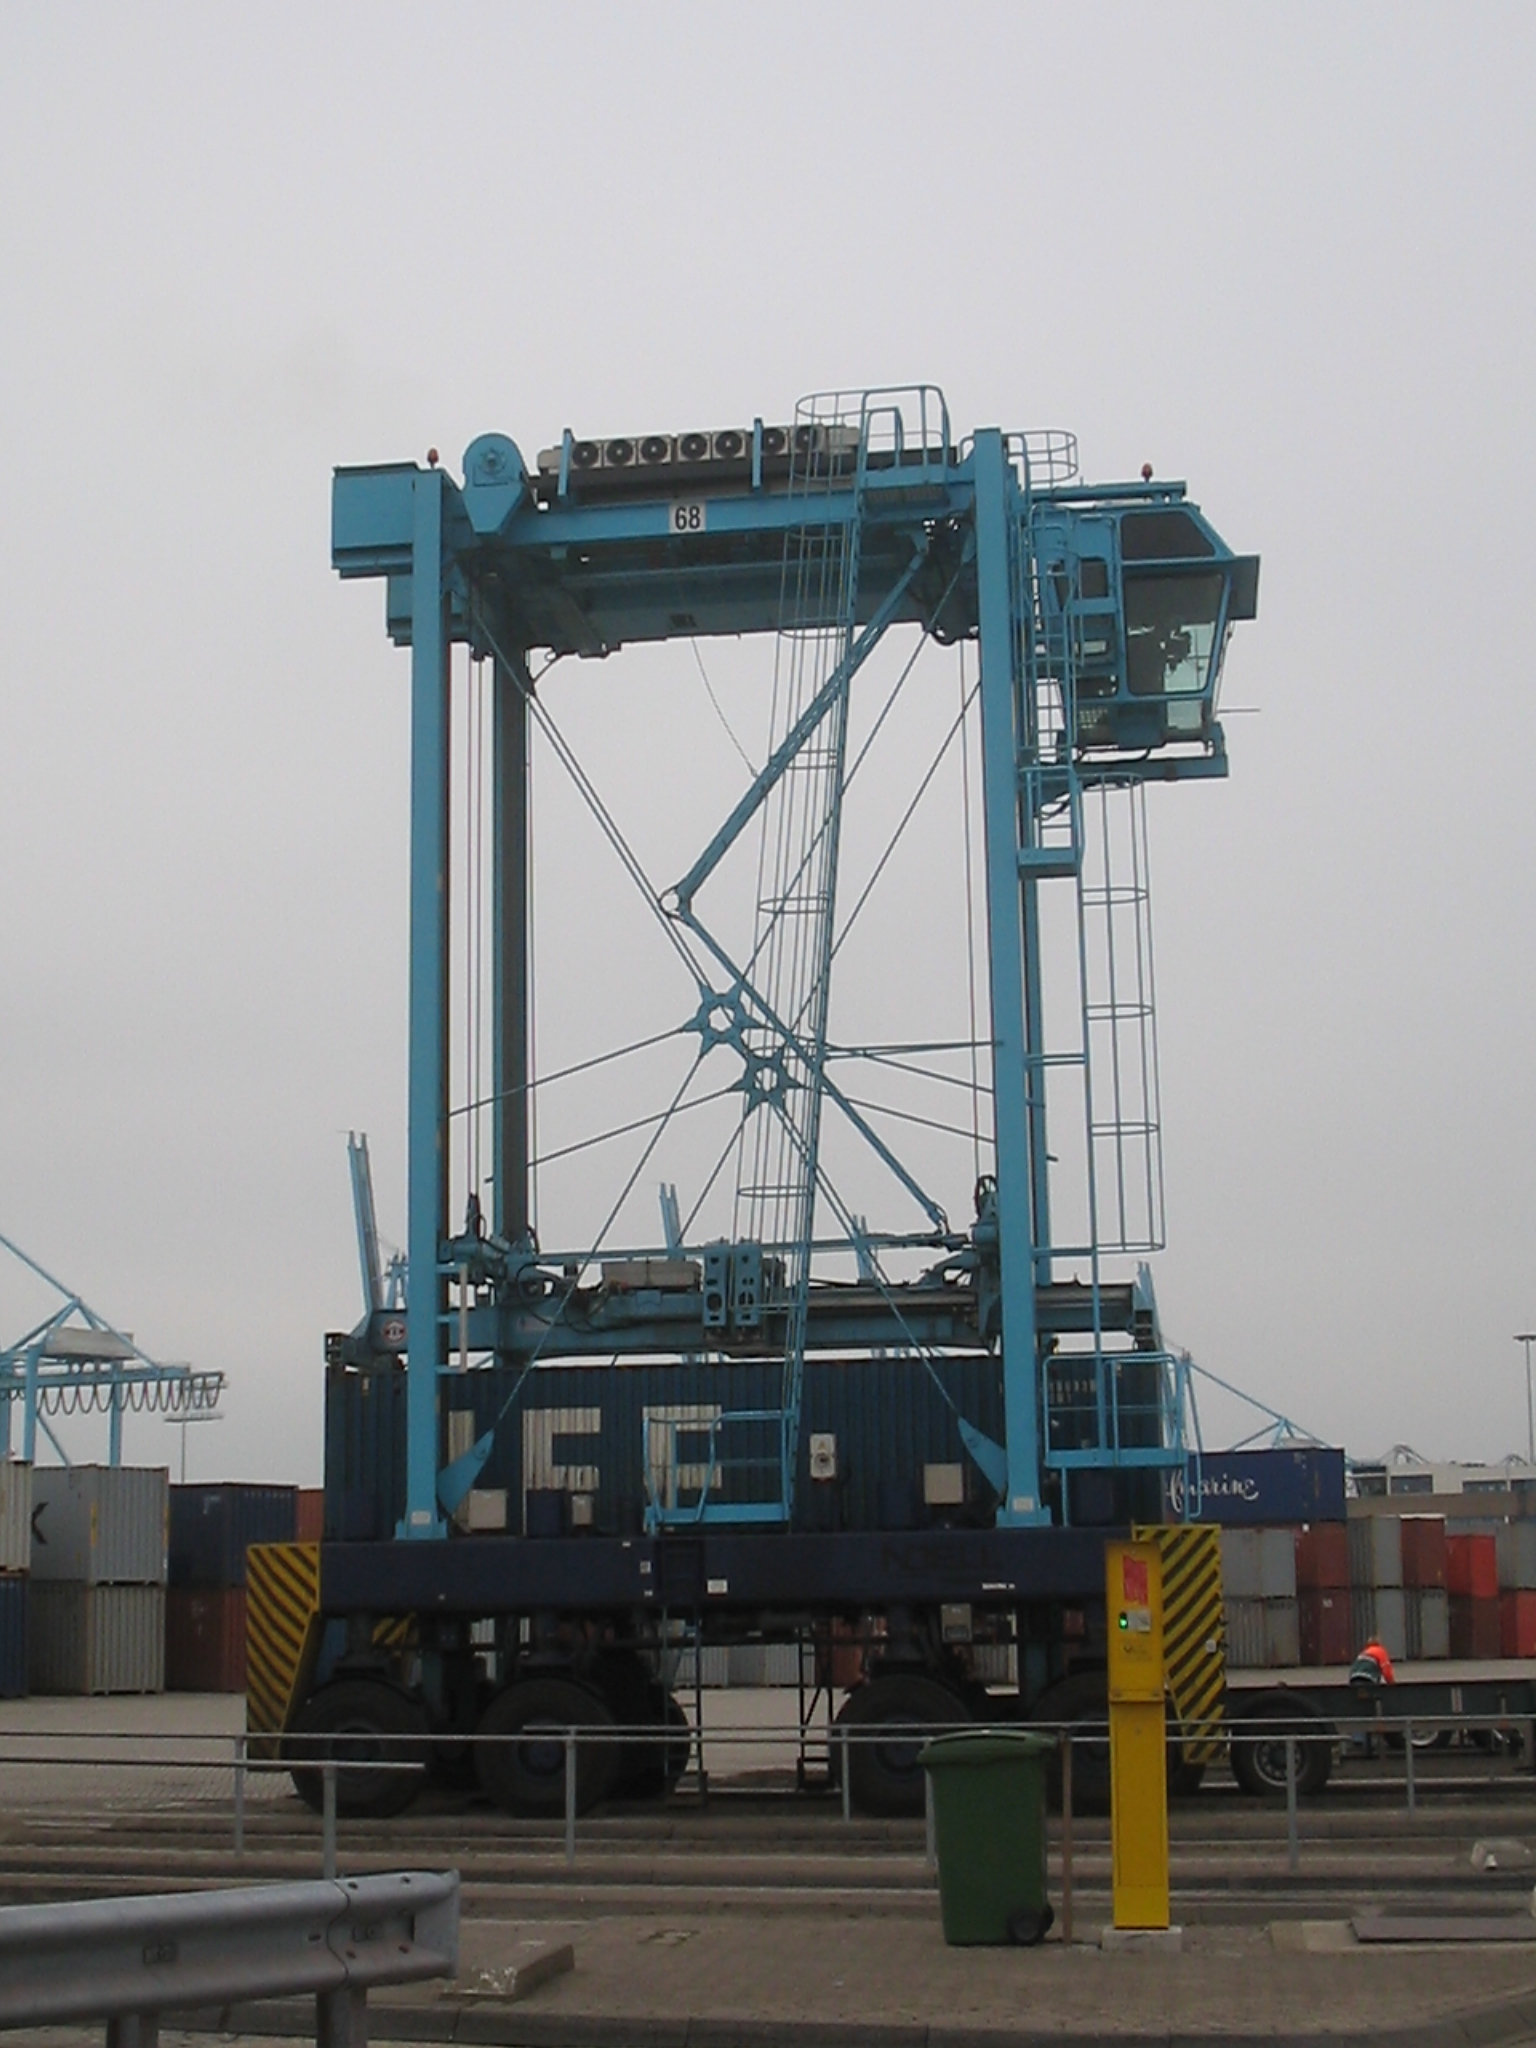
\includegraphics[height=.4\textheight]{../Articles/Figures/Containerlift_straddle_carrier.jpg}
			\end{flushright}
		\end{column}
 	\end{columns}

	
\end{frame}
\subsection*{Dynamic of the system}
\begin{frame}
\frametitle{System dynamic}
	\begin{columns}
		\begin{column}[l]{8cm}
			\begin{itemize}
				\item Open system means uncertain environment
				\item 3 kinds of unpredictable events : 
				\begin{itemize}
 					\item Incoming missions
					\item Trucks arriving time
					\item Human behavior
				\end{itemize}
			\end{itemize}
		\end{column}
		\begin{column}[r]{4cm}
			\begin{center}
				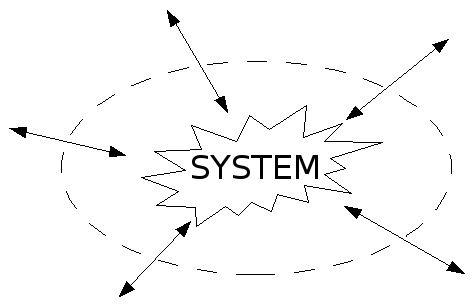
\includegraphics[height=.30\textheight]{../Articles/Figures/openSystem.png}
			\end{center}
	 	\end{column}
	\end{columns}
\end{frame}

\section{Vehicle Routing Problem : state of the art}

\subsection*{Vehicle Routing Problem with Time Windows}

\begin{frame}
\frametitle{VRPTW\cite{Berbeglia07}}
	\begin{columns}
	 	\begin{column}[l]{6cm} \begin{center}
			\begin{itemize}
 				\item \textbf{V}ehicle \textbf{R}outing \textbf{P}roblem
			\end{itemize} \end{center}
	 	\end{column}
	 	\begin{column}[r]{6cm} \begin{center}
			\begin{itemize} 
				\item \textbf{T}ime \textbf{W}indows
			\end{itemize} \end{center}
	 	\end{column}
	\end{columns}
	\begin{block}{Goal}
		\begin{center} Optimizing the delivery routes of each truck \end{center}
	\end{block}
		
	\begin{exampleblock}{example of VRPTW : the Italian factory}
		\begin{itemize}
			\item The factory produces toys and its vehicles deliver a set of stores
			\item Stores are spread all over the country and goods are carried by trucks
			\item Every truck has a restricted capacity and starts from the factory depot
			\item Deliveries must occur during a time interval and if a truck comes too early, it will have to wait
		\end{itemize}
	\end{exampleblock}
\end{frame}


\subsection*{Dynamic Vehicle Routing Problem with Time Windows}
\begin{frame}
	\frametitle{DVRPTW\cite{Mitrovic01}}
	\begin{itemize}
 		\item Dynamic
	\end{itemize}
	\begin{block}{Goal}
		\begin{center}
			Optimizing the new routes of each truck without recomputing from scratch
		\end{center}
	\end{block}	
	
	\begin{exampleblock}{Dynamic Italian factory}
		\begin{itemize}
			\item Italian factory problem
			\item While a schedule is running, stores are still allowed to ask for a delivery
		\end{itemize}
	\end{exampleblock}
\end{frame}

\subsection*{(Dynamic) Pickup and Delivery Problem}
\begin{frame}
 \frametitle{(D)PDP}
	\begin{itemize}
	 \item DVRP where the goods have to be picked-up before being delivered
	\end{itemize}
	
	\begin{block}{Goal}
		\begin{center}
			Optimizing both pickup and delivery routes
		\end{center}
	\end{block}	
	\begin{exampleblock}{Pickup and Delivery Problem example : mail delivery problem}
		\begin{itemize}
			\item A mail company employs a set of postmen
			\item They have to pickup mails from the mail boxes of the company
			\item Then, they must deliver them to their recipients as soon as possible
		\end{itemize}
	\end{exampleblock}

\end{frame}

\subsection*{Dynamic Straddle Carriers Pickup and Delivery Problem with Time Windows}
\begin{frame}
\frametitle{DSCPDPTW}
	\begin{itemize}
 		\item Dynamic Pickup and Delivery Problem class
		\item Vehicles can start from anywhere - they do not have to start from the depot
	\end{itemize}

	\begin{itemize}
	 \item 2 problems : 
		\begin{itemize}
 			\item Minimize straddle carriers moves : shortest path problem
			\item Minimize customers delays : scheduling problem
		\end{itemize}
	\end{itemize}
	
	
	\begin{alertblock}{Problem dependencies}
		\begin{tabular}{*{3}{l}}
			appropriate scheduling & $\Rightarrow$ & shortest path concept\\
			scheduling shortest paths & $\Rightarrow$ & reducing straddle carriers moves
		\end{tabular}
	\end{alertblock}

	\begin{block}{Goal}
		\begin{center}
		Solving these 2 interconnected problems
		\end{center}
	\end{block}	

\end{frame}


\section{Ant Colony and Straddle Carrier Handling}
\subsection*{Ant Colony : general description}
\begin{frame}
\frametitle{Ant Colony Optimization\cite{Dorigo91}}
	\begin{itemize}
 		\item ACO is a meta-heuristic
		\item ACO makes a solution appear thanks to the run of artificial ants into the solution space
		\item ACO is adapted to the dynamic nature of this problem :
		\begin{itemize}
		     \item Positive feedback : ants spread pheromone according to solution quality
		     \item Negative feedback : pheromone track evaporates progressively
		\end{itemize}

	\end{itemize}
	
\end{frame}
\subsection*{Ant Colony and scheduling}
\begin{frame}
\frametitle{Scheduling with Ant Colony}
 	
	Ant Colony with \textbf{one colony} provides a sorted list of missions to accomplish.
	\pause
	\begin{block}{Problem}
		\begin{center}
			How to set a mission to a specific straddle carrier ?
		\end{center}
	\end{block}

	
	\pause
	\begin{block}{Colored ants\cite{Bertelle02} : }
	\begin{itemize}
 		\item every straddle carrier represents a colony with its own color
		\item ants are attracted by pheromones of their own colony
		\item ants are repulsed by pheromones of foreign colonies
	\end{itemize}
	\end{block}
	\pause
	Ant Colony with \textbf{many colonies} provides a sorted list of missions per straddle carrier.
	
\end{frame}
\subsection*{Scheduling modeling : missions graph}
\begin{frame}
\frametitle{Missions graph}
	The directed graph can be conceptualized as follows :
		\begin{itemize}
	 		\item Vertices : 
				\begin{itemize}
 					\item 1 mission = 1 node
					\item 1 straddle carrier = 1 colored node connected to all compatible missions
				\end{itemize}
 
			\item Colored Arcs :
				\begin{itemize}
					\item Compatibility between 2 missions for a straddle carrier
				\end{itemize}
		\end{itemize}

	\begin{block}{Ordering missions}
		We say that mission $m_a$ is \textbf{prior} to mission $m_b$ if the time window of $m_a$ starts before the one of $m_b$
	\end{block}

	\begin{block}{Mission compatibility}
		We say that mission $m_a$ is \textbf{compatible} with mission $m_b$ if $m_a$ is prior to $m_b$
	\end{block}

\end{frame}
\begin{frame}
 \frametitle{Example of a mission graph construction (1)}
	\begin{exampleblock}{Example}
		\begin{itemize}
		 \item Missions : \\
		\begin{center}
			\begin{tabular}{*{3}{|c|c|c}}
	 	 		\hline
		 		Name	&	Start	&	End\\
				\hline
				m0	&	5:00	&	6:00 \\
				m1	&	5:30	&	6:00 \\
				m2	&	7:00	&	9:00 \\
				m3	&	6:00	&	7:30 \\
				\hline
	 		\end{tabular}
		\end{center}
		\item Straddle Carriers : \\
		\begin{center}
			\begin{tabular}{*{3}{|c|c|c}}
	 	 		\hline
		 		Name	&	Color	& Compatiblility\\
				\hline
				s0	&	\textcolor{green}{green}	& m0, m1, m2, m3\\
				s1	&	\textcolor{blue}{blue}	& m0,m3\\	
				\hline
	 		\end{tabular}
		\end{center}
		
		\end{itemize}

	\end{exampleblock}
	

	
\end{frame}
\begin{frame}
	\frametitle{Example of a mission graph construction (2)}
	\begin{center}
		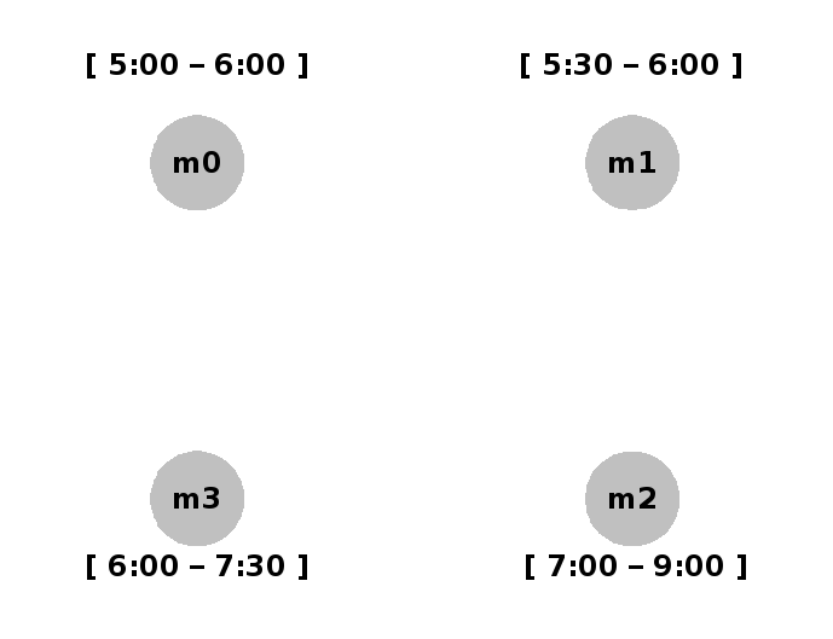
\includegraphics[height=.50\textheight]{../Articles/Figures/only_vertices.png} \\
	
		1 mission $\Longleftrightarrow$ 1 vertex
	\end{center}
	
\end{frame}
\begin{frame}
	\frametitle{Example of a mission graph construction (3)}
 	\begin{center}
 		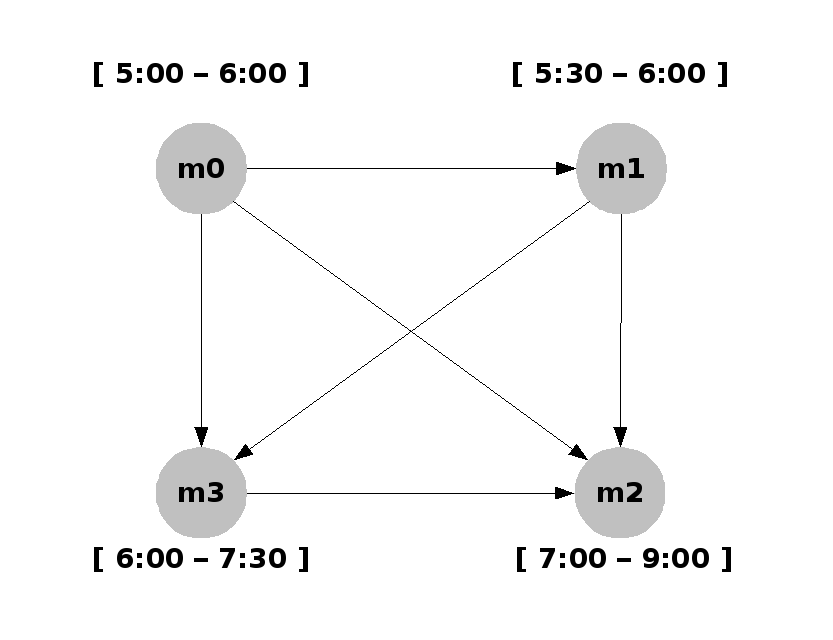
\includegraphics[height=.50\textheight]{../Articles/Figures/precedence.png} \\

		1 arc between two compatible missions
	\end{center}
\end{frame}
\begin{frame}
	\frametitle{Example of a mission graph construction (4)}
 	\begin{center}
 		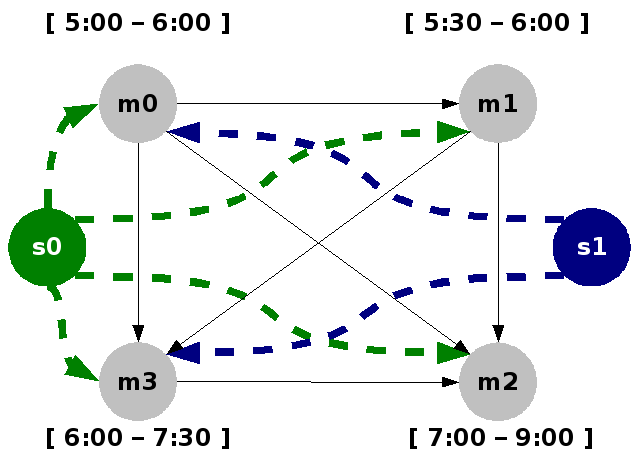
\includegraphics[height=.50\textheight]{../Articles/Figures/precedence_with_vehicles.png}
		
		Adding nodes modeling straddle carriers and connecting them to every other vertices
	\end{center}
\end{frame}
\begin{frame}
	\frametitle{Example of a mission graph construction (5)}
 	\begin{center}
 		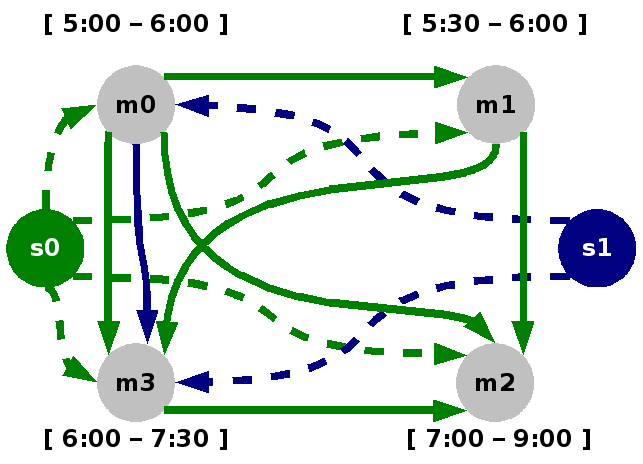
\includegraphics[height=.50\textheight]{../Articles/Figures/missionGraphComplet.png}
		
		Adding or Coloring edges between nodes according to their connectivity with the vehicles
	\end{center}
\end{frame}
\subsection*{Main algorithm}

\begin{frame}
\frametitle{Algorithm description}
	\setbeamertemplate{blocks}[rounded][shadow=true]
	\begin{block}{Main algorithm}
	\underline{begin}\\
	$\vert \;$\underline{for} each colony $c$ \underline{do}\\
	$\vert \;\vert \;$\underline{for} each ant $a$ of $c$ \underline{do}\\
	$\vert \;\vert \;\vert \;$choose an unvisited destination according to the pheromone track\\
	$\vert \;\vert \;\vert \;$move towards it according to the speed of $a$\\
	$\vert \;\vert \;\vert \;$spread pheromone according to the destination quality\\
	$\vert \;\vert \;$\underline{end for}\\
	$\vert \;$\underline{end for}\\
	$\vert \;$evaporation\\
	\underline{end}\\
	\end{block}
\end{frame}
\subsection*{Solution}
\begin{frame}
\frametitle{Solution}

	\begin{itemize}
	  \item The solution is the coloring of the nodes.
	  \item When a straddle carrier is free, it chooses the mission of its color which has the highest pheromone rate.
	  \item The chosen missions are removed from the graph and the algorithm continues running.
	\end{itemize}
	
	\begin{center}
		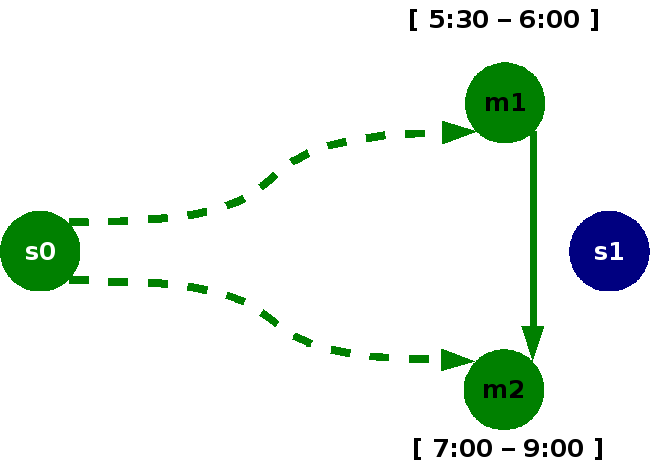
\includegraphics[height=.50\textheight]{../Articles/Figures/missionGraphWith2NodesRemoved.png}
	\end{center}
\end{frame}
\section{Simulator}
\subsection*{2 parallel views of the system}
\begin{frame}
\frametitle{2 parallel views of the system}
	\setbeamertemplate{blocks}[rounded][shadow=true]
 	\begin{columns}
	 	\begin{column}[l]{6cm}
	 		\begin{itemize}
				 \item Terminal implementation
			\end{itemize}
		\end{column}
		\begin{column}[r]{6cm}
			\begin{itemize}
				  \item ACO modeling\cite{Dutot2007}
			\end{itemize}
		\end{column}
 	\end{columns}
	\begin{center} 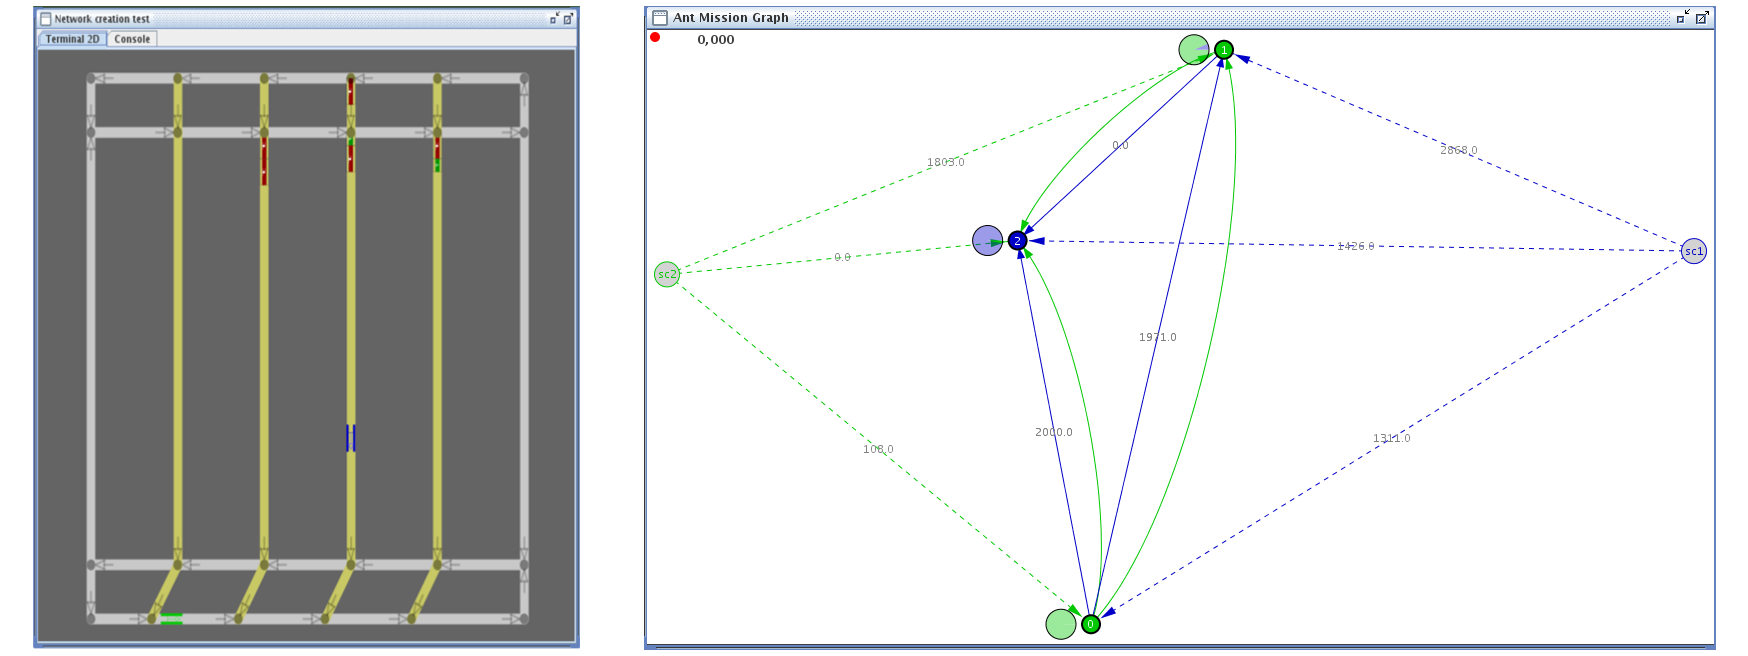
\includegraphics[height=3.7cm]{../Articles/Figures/terminalEtGraphe.png} \end{center}

	\begin{block}{ACO $\Longleftrightarrow$ Terminal}
		\begin{center}
			Effects of ACO results must appear on the terminal and the terminal state must affect the ACO setting (mission graph)
	 	\end{center}
	\end{block}
\end{frame}
\subsection*{Dynamism handling}
\begin{frame}

 \frametitle{Dynamism handling}
A scenario file is read all along the execution of the simulation. It contains dynamic events.

\begin{block}{Measure of dynamism}
According to A. Larsen\cite{Larsen00}, we can measure how dynamic is a scenario by these two formulas : 
  \begin{itemize}
  \item Degree of Dynamism (dod) = $\frac{\eta_d}{\eta_s+\eta_d}$
  \item Effective Degree of Dynamism (edod) = $\; \frac{\sum_{i=1}^{\eta_d}\frac{t_i}{T}}{\eta_s+\eta_d}$
\end{itemize}

$\eta_s$ : number of static requests ; \\
$\eta_d$ : number of dynamical requests.

\end{block}
\end{frame}


\section{Preliminary Results}
\begin{frame}
\frametitle{Preliminary results}
\begin{itemize}
 \item Test the relevance of both our modeling and our algorithm on simulated data
 \item Function of the measures of dynamism
\end{itemize}

\begin{center}
	\begin{tabular}{*{5}{|l|c|c|c}}
		\hline
						& Static& Half Dynamic & Dynamic \\
		\hline
		$dod$				& 0 	&0.5 	& 1 	 \\
		$edod$				& 0 	&0.25	& 1 	\\
		\hline
		End time 			&22693	& 22276	& 22693   \\
		\hline		
		Number of overrun tw		&3	&5 	& 7 \\
		\hline		
		Overrun time penalty		&6467	&8477	& 12485\\
		\hline
	
	\end{tabular}
\end{center}

%Comment
The exceeded time windows and the time penalties evolve in the same way that $dod$ and $edod$.

\end{frame}

\section{Conclusion}
\begin{frame}
 \frametitle{Conclusion}
	\begin{itemize}
	 \item The problem to solve belongs to the Dynamic Pickup and Delivery Problem with Time Windows class
	 \item It does not totaly fit, so it is an original and unsolved problem
	 \item Swarm intelligence has been used to solve it, containing :
	 \begin{itemize}
		\item Ant Colony System
		\item Colored Ants
		\item A Graph modeling
	\end{itemize}
	 \item A simulator is being developped and will allow to measure the solution relevance
	 \item Priliminary results confirm that our modelling is able to handle dynamics
	\end{itemize}

	\pause
	\begin{center}
		\textbf{Thank you for your attention}
	\end{center}

\end{frame}
\tiny
\bibliographystyle{plain}
\bibliography{../Articles/Bibliography/biblio}
% \begin{frame}
%  \frametitle{UML modeling}
% 	\begin{figure}[center,h]
% 		\includegraphics[height=0.8\textheight]{Shemas/simplified_uml.png}
% 	\end{figure}
% \end{frame}
% 
% 
% \begin{frame}
%  \frametitle{UML modeling}
% 		\begin{figure}[center,h]
% 			\includegraphics[height=0.8\textheight]{Shemas/uml_aco.png}
% 		\end{figure}
% \end{frame}
\end{document}